\begin{figure}[h!]
    \centering
    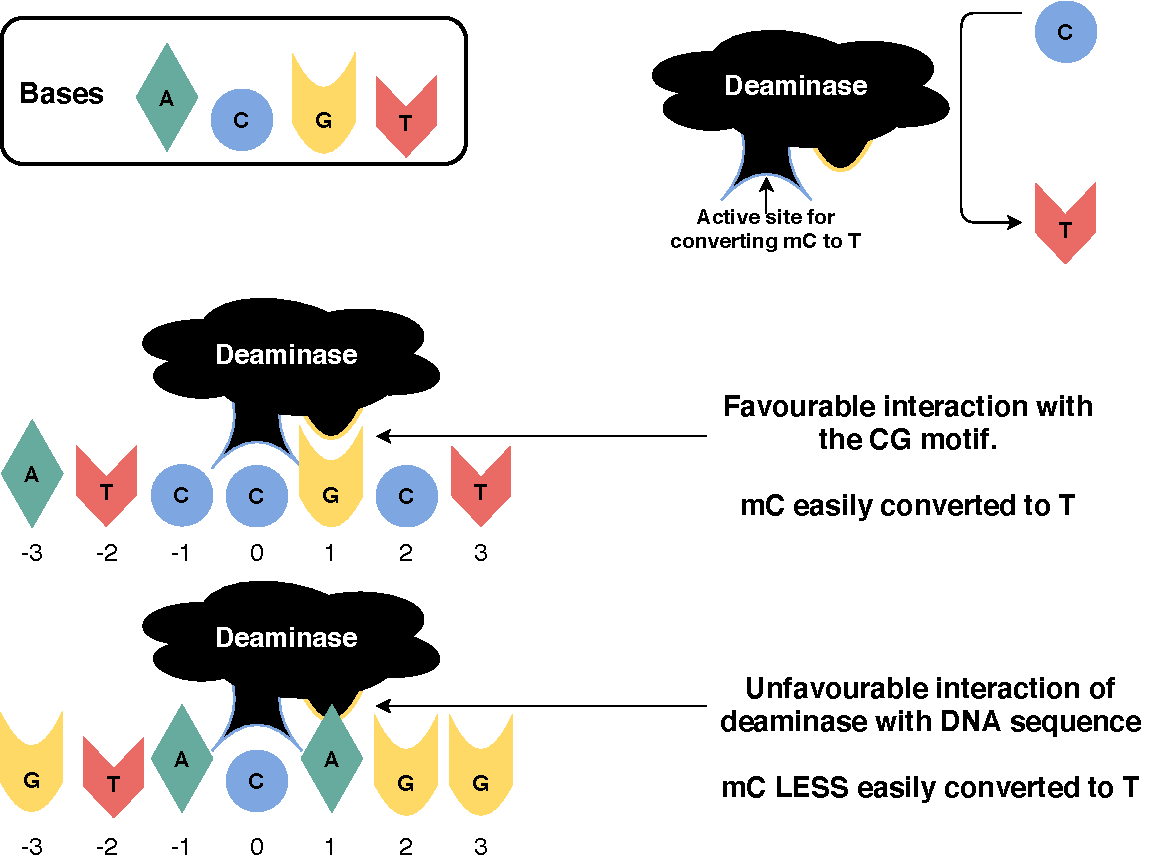
\includegraphics[scale=0.78]{graphics/motif_demo.pdf}
    \caption{\textbf{Mutations are closely linked with the bases next to them}. The schematic diagram depicts an example of hypothetical scenarios that could explain why this is the case. Here, methyltransferase, which methylates C into mC, interacts with DNA such that certain sequence contexts make the conversion more feasible. mC is an ``excited'' state that is prone to the C$\rightarrow$T mutations. While many publications focus on the 3-mer context of mutations (pos -1, 0 and 1), which includes the base change and two bases immediately next to it, evidence shows that bases outside the 3-mer could still be influential. Additionally, mutations tend to be considered equivalent to their reverse complementary counterparts in a strand symmetric manner (\textit{e.g.} G$\rightarrow$A and C$\rightarrow$T), but observations supporting strand asymmetry have been reported. Part of this project seeks to explore the information content available in larger sequence contexts than 3-mers. Another part explores the effect of the strand symmetric \textit{v.s.} strand asymmetric representations.}
    \label{fig:motif_demo}
\end{figure}
